\begin{comment}
\begin{table*}[ht!]
\centering
\begin{tabular}{|c|c|c|c|c|}
\hline
\textbf{VCA} & \textbf{Platforms}     & \textbf{Encoding} & \textbf{Direct connection?} & \textbf{Network Protocol} \\ \hline
\hline 
Meet  & Browser, Phone         & VP9/VP8   & No                 & RTP (WebRTC)     \\ \hline
Teams & Native, Browser, Phone & VP9       & ?                  & RTP              \\ \hline
Zoom  & Native, Browser, Phone & H.264 SVC & Yes                & Variation of RTP \\ \hline
\end{tabular}
\caption{Design parameters of selected VCAs}
\label{tab:vca_overview}
\end{table*}
\end{comment}
\section{Background and Setup}

\begin{figure}[h]
\centering
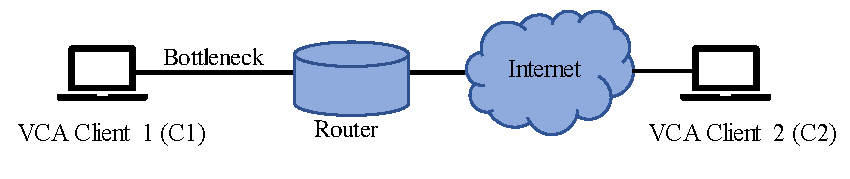
\includegraphics[width=0.45\textwidth,keepaspectratio]{methodology/normal-setup.pdf}
\caption{Setup for 2-person call}
\label{fig:static_setup}
\end{figure}


\label{sec:background}
Most VCAs use Real-time Transport Protocol (RTP)~\cite{schulzrinne1996rtp, schulzrinne2003rfc3550} or its variants~\cite{baugher2004secure, zoom_rtp} to transmit media content. The audio and video data is generally transmitted over separate RTP connections. RTP also uses two other protocols in conjunction, Session Initiation Protocol (SIP)~\cite{rosenberg2002sip} to establish connection between clients and RTP Control Protocol (RTCP)~\cite{schulzrinne2003rfc3550} to share performance statistics and control information during a call. Despite using well-known protocols, VCAs can differ from each other significantly across the following dimensions:



\textbf{Network mechanisms}: RTP and the associated protocols are implemented in the application-layer. Thus, the specific implementation of the protocols can vary across VCAs. For instance, Zoom reportedly uses a custom extension of RTP~\cite{zoom_rtp}). Furthermore, the key network functions, i.e., congestion control and error recovery, are also implemented in the application-layer as RTP runs over UDP.

\textbf{Application-layer parameters}: These include media encoding standards and default bitrates. More recent video codecs (e.g., VP9, H.264) can encode at the same video quality with fewer bytes when compared to older codec (e.g., VP8), albeit with a higher compute overhead~\cite{bienik2016performance}. % The audio data is encoded using constant-bitrate. Video is encoded using standard codecs such as VP9 and H.264 with the bitrate controlled based on the underlying network conditions.

\textbf{Streaming architecture}: VCAs can either choose to use direct or peer-to-peer connections or use relay servers. Centralized servers are almost always used for multi-point calls to combine data from multiple users. VCAs can differ in the exact strategies of data combination as well as the geographic footprint of their servers. For instance, Zoom rapidly expanded its server infrastructure to support increased call volume because of COVID-19~\cite{liu2020characterizing}. 


Differences across one or more of these factors can lead to different network utilization and performance. In this paper, we aim to dig deeper into these differences for a subset of VCAs. 

% use P2P or a relay server. STUN servers used to by pass NAT. TURN servers are used for multi-party calls or when a direct connection cannot be established. In some cases, using a relay server can also improve performance~\cite{via}.

% \textbf{Networking mechanisms}: These include important functions such as congestion control and error correction mechanisms. VCAs have their own proprietary implementations of these mechanisms. 

%\textbf{Application-layer parameters}: 

%\textbf{Video conferencing architecture}: Direct vs relay-based. Also differ in the capabilities of the relaying server. 




% Thus, the logic for congestion control is implemented in the application-layer. Audio and video data are usually transmitted over separate RTP channels. T RTCP is the control channel that provides end-to-end feedback about the network. 






\subsection{Setup}



We conduct experiments in a controlled environment. We now describe our experiment setup for a 2-party call (see Figure~\ref{fig:static_setup}. We use two identical
Dell Latitude 3300 laptops with a screen resolution of 1366 $\times$ 768 pixels and running Ubuntu 20.04.1. The laptops have a wired connection to a Turris Omnia 2020
router and access an unconstrained 1-gigabit link to the public Internet. Each experiment consists of initiating a n-seconds call between the two machines under a
pre-specified network bandwidth profile and VCA. We emulate a variety of network conditions on the \textit{C1-router} link using traffic control (\texttt{tc}). A
pre-recorded talking-head video\footnote{Using the device webcam feed is a non-starter because without movement, VCAs compress the video and ultimately send at a much
lower rate than during a normal call.} with a resolution of 1280 $\times$ 720 is used as the video source for the call. This is done to both replicate a real video call
and ensure consistency across experiments. All experiments are conducted with the laptop lid open and the application window maximized. % Run otherwise, the applications may adapt their behavior. [Tarun: not needed]


%on the laptop and router for uplink and downlink shaping, respectively. During the competition experiments, all shaping occurs at the router.

\textbf{Automating Calls}: To conduct a large number of experiments, we automated the entire in-call process. %It is crucial that the automated calls are as close to an actual call as possible, as any deviation from real call use may warp results. We take several steps to recreate the in-call process. 
We use the Python PyAutoGUI package~\cite{pyautogui} to automate joining and leaving calls. The package enables to programmatically control the keyboard and the mouse by specifying coordinates or visual elements on the screen. For \zoombrowser, we encountered CAPTCHA before joining a call on the default browser. Using the Selenium-based Chrome browser~\cite{selenium}, however, enabled us to bypass the CAPTCHA. Note the experiments using Selenium are run exactly as it would be in default Chrome browser. The entire workflow is controlled using a wrapper script on C1 with TCP sockets used to coordinate between C1 and C2. 




The setup is modified for later experiments (e.g., multi-party calls) and the modifications are described in the respective sections.


\subsection{VCA selection} 
We focus on three popular VCAs, namely \zoom, Google \meet, Microsoft \teams. These VCAs have been used extensively worldwide over the past year, especially in enterprises and educational institutions~\cite{vca_share}. Most of our experiment methodology, however, can be extended to other VCAs. We plan to make our code public to facilitate replication to other VCAs. %Table~\ref{tab:vca_overview} provides an overview of the design of the VCAs. 
All VCAs are tested in their native client unless otherwise indicated. Note, the application's ``native client'' refers to the Chrome browser for Meet and the desktop applications for Zoom and Teams. In the first set of experiments, we compare browser vs. client utilization for Teams and Zoom. In-browser tests will be specified by \textit{Teams-chrome} or \textit{Zoom-chrome}. We use Chrome (Meet) version 89.0.4389, Zoom client version 5.6.1, and Teams client version 1.4.00.7556.





\begin{comment}
\textbf{Performance metrics}: We mainly focus on the following application metrics. 
\begin{itemize}
    \item \textbf{Network bitrate}
    \item Video resolution
    \item Frames per second
    \item Freeze count
    \item Freeze duration
    \item Jitter-buffer delay 
\end{itemize}

Most of our analysis is using network bitrate. We consider other application performance metrics when they can be extracted from Google Chrome\footnote{chrome://webrtc-internals}. Our analysis shows that there is a strong correlation between network bitrate and application performance. This is intuitive as real-time streaming is characterized by low latency and thus any network interruptions usually lead to degradation in application performance. 


\subsection{Measurement Methodology}
  
The measurement setup consists of several components:

Hardware
\begin{itemize}
    \item matched laptops for nominal flows
          \begin{itemize}
              \item All Linux; caveats -- may not be the most-maintained apps
              \item What laptops, for the many-laptop tests?
          \end{itemize}
    \item turris router for control of single shaped link
    \item private iperf server on university network
\end{itemize}

\begin{itemize}
    \item traffic control scripts
    \item autogui; selenium for browser
          \begin{itemize}
              \item Important that we have the screen up -- see e.g., the tweet, but maybe chase the paper, about the struggle of getting the machines to actually render flows being important.
              \item client vs browser
              \item sw versions?
          \end{itemize}
    \item pcap, iperf logs
    \item webrtc
          \begin{itemize}
              \item difference between meet and zoom 
          \end{itemize}
    \item Zoom API access (\& limitations?)
    \item control over sockets?
\end{itemize}
\end{comment}